\chapter{Calculations of $\pi_1(X)$}

\section*{12.3.1. Some basic results on \({\pi }_{1}\left( {X,b}\right)\)}

We will study \({\pi }_{1}\left( {X,b}\right)\) for some simplicial complexes.

Definition 12.2 [Edge Loop] Let \(K = \left( {V,\sum }\right)\) be a simplicial complex.

1. An edge path \(\left( {{v}_{0},\ldots ,{v}_{n}}\right)\) is such that

(a) \({a}_{i} \in  V\left( K\right)\)

(b) For each \(i,\left\{  {{a}_{i - 1},{a}_{i}}\right\}\) spans a simplex of \(K\)

2. An edge loop is an edge path with \({a}_{n} = {a}_{0}\) .

3. Let \(\alpha  = \left( {{v}_{0},\ldots ,{v}_{n}}\right) ,\beta  = \left( {{w}_{0},\ldots ,{w}_{m}}\right)\) be two edge paths with \({v}_{n} = {w}_{0}\) , then we define

\[
\alpha  \circ  \beta  = \left( {{v}_{0},\ldots ,{v}_{n},{w}_{1},\ldots ,{w}_{m}}\right)
\]

Definition 12.3 [Elementary Contraction/Expansion] Let \(\alpha ,\beta\) be two edge paths.

1. An elementary contraction of \(\alpha\) is a new edge path obtained by performing one of the followings on \(\alpha\) :

\begin{itemize}
\item Replacing \(\cdots {a}_{i - 1}{a}_{i}\cdots\) by \(\cdots {a}_{i - 1}\cdots\) provided that \({a}_{i - 1} = {a}_{i}\)
\end{itemize}

\begin{itemize}
\item Replacing \(\cdots {a}_{i - 1}{a}_{i}{a}_{i + 1}\cdots\) by \(\cdots {a}_{i - 1}\cdots\) provided that \({a}_{i - 1} = {a}_{i + 1}\)
\end{itemize}

\begin{itemize}
\item Replacing \(\cdots {a}_{i - 1}{a}_{i}{a}_{i + 1}\cdots\) by \(\cdots {a}_{i - 1}{a}_{i + 1}\cdots\) provided that \(\left\{  {{a}_{i - 1},{a}_{i},{a}_{i + 1}}\right\}\) spans a 2-simplex of \(K\) .
\end{itemize}

2. An elementary expansion is the reverse of the elementary contraction.

3. Two edge paths \(\alpha ,\beta\) are equivalent if \(\alpha\) and \(\beta\) differs by a finite sequence of elementary contractions or expansions.

\section*{12.6. Wednesday for MAT4002}

Reviewing.

\begin{itemize}
\item Edge loop based at \(b \in  V\) :
\end{itemize}

\[
\alpha  = \left( {b,{v}_{1},\cdots ,{v}_{n},b}\right)
\]

\begin{itemize}
\item Equivalence class of edge loops:
\end{itemize}

\[
\left\lbrack  \alpha \right\rbrack   = \left\{  {{\alpha }^{\prime } \mid  {\alpha }^{\prime } \sim  \alpha ,{\alpha }^{\prime }\text{ is the edge loop based at }b}\right\}
\]

Note that \({\alpha }^{\prime } \sim  \alpha\) if they differ from finitely many elementary contractions or expansions.

For instance, let \(K\) in the figure below denote a triangle:

\begin{center}
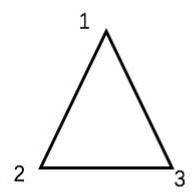
\includegraphics[max width=0.2\textwidth]{images/bo_d2bcsrref24c73avs720_126_729_1128_194_194_0.jpg}
\end{center}
\hspace*{3em} 

Figure 12.1: Triangle \(K\)

Then the canonical form of any equivalence form \(\left\lbrack  \alpha \right\rbrack\) can be expressed as:

\[
\left\lbrack  \alpha \right\rbrack   = \left\lbrack  {{bcabc}\cdots {ab}}\right\rbrack  ,
\]

where \(a,b,c \in  \{ 1,2,3\}\) are distinct.

\section*{12.6.1. Groups \& Simplicial Complices}

Proposition 12.7 The \(E\left( {K,b}\right)  = \{ \left\lbrack  \alpha \right\rbrack   \mid  \alpha\) is edge loop based at \(b\}\) is a group, with the operation

\[
\left\lbrack  \alpha \right\rbrack   * \left\lbrack  \beta \right\rbrack   = \left\lbrack  {\alpha  \cdot  \beta }\right\rbrack
\]

\[
\alpha  \sim  {\alpha }^{\prime },\beta  \sim  {\beta }^{\prime } \Rightarrow  \alpha  \cdot  \beta  \sim  {\alpha }^{\prime } \cdot  {\beta }^{\prime }
\]

2. Associativity is clear.

3. The identity is \(e \mathrel{\text{ := }} \left\lbrack  b\right\rbrack\) : for any edge loop \(\left\lbrack  \alpha \right\rbrack   = \left\lbrack  {b{v}_{1}\cdots b}\right\rbrack\) ,

\[
\left\lbrack  \alpha \right\rbrack   * e = \left\lbrack  {b{v}_{1}\cdots {v}_{n}b}\right\rbrack   * \left\lbrack  b\right\rbrack
\]

\[
= \left\lbrack  {b{v}_{1}\cdots {v}_{n}{bb}}\right\rbrack
\]

\[
= \left\lbrack  {b{v}_{1}\cdots {v}_{n}b}\right\rbrack   = \left\lbrack  \alpha \right\rbrack  .
\]

Also, \(e * \left\lbrack  \alpha \right\rbrack   = \left\lbrack  \alpha \right\rbrack\) .

4. The inverse of any edge loop \(\left\lbrack  {b{v}_{1}\cdots {v}_{n}b}\right\rbrack\) is \(\left\lbrack  {b{v}_{n}\cdots {v}_{1}b}\right\rbrack\) :

\[
{\left\lbrack  b{v}_{1}\cdots {v}_{n}b\right\rbrack  }^{-1} * \left\lbrack  {b{v}_{1}\cdots {v}_{n}b}\right\rbrack   = \left\lbrack  {b{v}_{n}\cdots {v}_{1}{bb}{v}_{1}\cdots {v}_{n}b}\right\rbrack
\]

\[
= \left\lbrack  {b{v}_{n}\cdots {v}_{1}b{v}_{1}\cdots {v}_{n}b}\right\rbrack
\]

\[
= \left\lbrack  {b{v}_{n}\cdots {v}_{2}{v}_{1}{v}_{2}\cdots {v}_{n}b}\right\rbrack
\]

\[
= \cdots
\]

\[
= \left\lbrack  b\right\rbrack
\]

Similarly, \(\left\lbrack  {b{v}_{1}\cdots {v}_{n}b}\right\rbrack   * {\left\lbrack  b{v}_{1}\cdots {v}_{n}b\right\rbrack  }^{-1} = \left\lbrack  b\right\rbrack\) .

We will see that for \(K\) defined in Fig.(12.1), \(E\left( {K,1}\right)  \cong  \mathbb{Z}\) , in the next class.

Theorem 12.5 \(E\left( {K,b}\right)  \cong  {\pi }_{1}\left( {\left| K\right| ,b}\right)\) .

This is the most difficult theorem that we have faced so far. Let's recall the simplicial approximation proposition first: Proposition 12.8 - Simplicial Approximation Proposition. Suppose that \(f\) : \(\left| K\right|  \rightarrow  \left| L\right|\) be such that for all \(v \in  V\left( K\right)\) , there exists \(g\left( v\right)  \in  V\left( L\right)\) satisfying

\[
f\left( {{\operatorname{st}}_{K}\left( v\right) }\right)  \subseteq  {\operatorname{st}}_{L}\left( {g\left( v\right) }\right) .
\]

As a result,

1. the mapping

\[
g : \;K \rightarrow  L
\]

\[
\text{ with }v \mapsto  g\left( v\right)
\]

is a simplicial map, i.e., for all \({\sigma }_{K} \in  {\sum }_{K},g\left( {\sigma }_{K}\right)  \in  {\sum }_{L}\)

2. Moreover, \(\left| g\right|  \simeq  f\) .

Furthermore, if \(A \subseteq  K\) is a simplicial subcomplex such that \(f\left( \left| A\right| \right)  \subseteq  \left| B\right|\) , where \(B \subseteq  L\) is a simplicial subcomplex, then we can choose \(g\) such that \({\left. g\right| }_{A} : A \rightarrow  B\) and the homotopy \(\left| g\right|  \simeq  f\) sends \(\left| A\right|\) to \(\left| B\right|\) .

\begin{itemize}
\item Example 12.8 Consider the simplicial complex \(K\) and \(L\) shown in the figure below:
\end{itemize}

\begin{center}
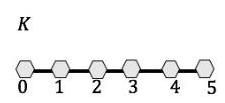
\includegraphics[max width=0.2\textwidth]{images/bo_d2bcsrref24c73avs720_128_422_1463_225_103_0.jpg}
\end{center}
\hspace*{3em} 

\begin{center}
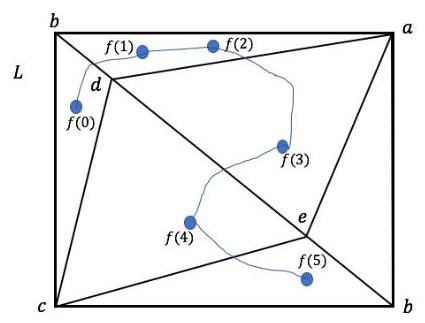
\includegraphics[max width=0.3\textwidth]{images/bo_d2bcsrref24c73avs720_128_830_1421_425_323_0.jpg}
\end{center}
\hspace*{3em} 

Let \({A}_{1}\) denote the subcomplex with \(V\left( {A}_{1}\right)  = \{ 0\} ,{\sum }_{{A}_{1}} = \{ \{ 0\} \}\) , and \({A}_{2}\) denote the subcomplex wit \(V\left( {A}_{2}\right)  = \{ 1,2\}\) and \({\sum }_{{A}_{2}} = \{ \{ 1,2\} ,\{ 1\} ,\{ 2\} \}\) . Therefore,

\[
f\left( \left| {A}_{1}\right| \right)  \subseteq  \left| {\Delta }_{\{ b,c,d\} }\right| ,\;f\left( \left| {A}_{2}\right| \right)  \subseteq  \left| {\Delta }_{\{ a,b,d\} }\right| ,
\]

There exists simplicial mapping \(g\) with

\[
g\left( 0\right)  = b,\;g\left( 1\right)  = b,\;g\left( 2\right)  = d,\;g\left( 3\right)  = e,\;g\left( 4\right)  = c,\;g\left( 5\right)  = c
\]

Proof. 1. For each edge loop \(\alpha  = \left( {{v}_{0},\ldots ,{v}_{n}}\right)\) based at \(b\) , consider the simplicial complex

\begin{center}
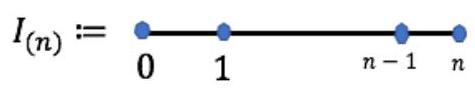
\includegraphics[max width=0.4\textwidth]{images/bo_d2bcsrref24c73avs720_129_718_891_475_90_0.jpg}
\end{center}
\hspace*{3em} 

Together with the simplicial map

\[
{g}_{\alpha } : \;{I}_{\left( n\right) } \rightarrow  K
\]

\[
\text{ with }{g}_{\alpha }\left( i\right)  = {v}_{i}
\]

Note that it is well-defined since \(\{ i,i + 1\}  \in  {\sum }_{{I}_{\left( n\right) }}\) , and \(\left\{  {{v}_{i},{v}_{i + 1}}\right\}   \in  {\sum }_{K}\) .

Now construct the mapping

\(\theta  : \;\{\) edge loop based at \(b\}  \rightarrow  {\pi }_{1}\left( {K,b}\right)\)

with \(\alpha  \mapsto  \left\lbrack  \left| {g}_{\alpha }\right| \right\rbrack\)

where \(\left| {g}_{\alpha }\right|  : \left| {I}_{\left( n\right) }\right| \left( { \cong  \left\lbrack  {0,1}\right\rbrack  }\right)  \rightarrow  \left| K\right|\)

\(\left| {g}_{\alpha }\right| \left( {i/n}\right)  = {v}_{i}\)

For example,

\[
\alpha  = \left( \text{ bdeab cb }\right) , \Rightarrow  \left| {g}_{\alpha }\right| \left( 0\right)  = b,\left| {g}_{\alpha }\right| \left( {1/6}\right)  = d,\left| {g}_{\alpha }\right| \left( {2/6}\right)  = e,\cdots ,\left| {g}_{\alpha }\right| \left( 1\right)  = b,
\]

i.e., \(\left| {g}_{\alpha }\right|\) is a loop based at \(b\) .

Therefore, \(\left\lbrack  \left| {g}_{\alpha }\right| \right\rbrack   \in  {\pi }_{1}\left( {\left| K\right| ,b}\right)\) .

2. Now, suppose \(\alpha  \sim  {\alpha }^{\prime }\) be two edge loops differ by an elemenary contraction, e.g.,

\[
{\alpha }^{\prime } = \left( \text{ bdebcb }\right)  \sim  \alpha  = \left( \text{ bdeabcb }\right) .
\]

As a result, \(\left| {g}_{{\alpha }^{\prime }}\right|  \simeq  \left| {g}_{\alpha }\right|\) relative to \(\{ 0,1\}\) , i.e., \(\left\lbrack  \left| {g}_{\alpha }\right| \right\rbrack   = \left\lbrack  \left| {g}_{{\alpha }^{\prime }}\right| \right\rbrack\) .

Therefore, we have a well-defined map:

\(\widetilde{\theta } : \;\{\) edge loops based at \(b\} / \sim   \rightarrow  {\pi }_{1}\left( {\left| K\right| ,b}\right)\)

with \(\left\lbrack  \alpha \right\rbrack   \mapsto  \left\lbrack  \left| {g}_{\alpha }\right| \right\rbrack\)

Therefore, \(\widetilde{\theta } : E\left( {K,b}\right)  \rightarrow  {\pi }_{1}\left( {\left| K\right| ,b}\right)\) is the desired map.

3. \(\widetilde{\theta }\) is a homomorphism: it suffices to show that

\[
\widetilde{\theta }\left( {\left\lbrack  \alpha \right\rbrack   * \left\lbrack  \beta \right\rbrack  }\right)  = \widetilde{\theta }\left( \left\lbrack  \alpha \right\rbrack  \right) \widetilde{\theta }\left( \left\lbrack  \beta \right\rbrack  \right) ,
\]

which suffices to show \(\left\lbrack  \left| {g}_{\alpha  \cdot  \beta }\right| \right\rbrack   = \left\lbrack  {\left| {g}_{\alpha }\right| \left| {g}_{\beta }\right| }\right\rbrack\) , i.e., \(\left| {g}_{\alpha  \cdot  \beta }\right|  \simeq  \left| {g}_{\alpha }\right| \left| {g}_{\beta }\right|\) . Note that \(\left| {g}_{\alpha  \cdot  \beta }\right|\) and \(\left| {g}_{\alpha }\right| \left| {g}_{\beta }\right|\) are the same path with different "speed", i.e., homotopy.

4. The mapping \(\widetilde{\theta }\) is surjective: Let \(\ell  : \left\lbrack  {0,1}\right\rbrack   \rightarrow  \left| K\right|\) be a loop based at \(b\) . It suffices to find an edge loop \(\alpha\) such that \(\left\lbrack  \left| {g}_{\alpha }\right| \right\rbrack   = \left\lbrack  \ell \right\rbrack\) , i.e., \(\left| {g}_{\alpha }\right|  \simeq  \ell\) .

(a) Applying the simplicial approximation theorem, there exist large \(n\) and \(g : {I}_{\left( n\right) } \rightarrow  K\) such that \(\left| g\right|  \simeq  \ell\) . Here we can choose \(g : {I}_{\left( n\right) } \rightarrow  K\) to be such that \(g\left( {\{ 0\} }\right)  = \{ b\} ,g\left( {\{ n\} }\right)  = \{ b\}\) , and \(\left| g\right|  \simeq  \ell\) relative to \(\{ 0,1\}\) .

(b) Take \(\alpha  = \left( {g\left( 0\right) ,g\left( 1\right) ,\ldots ,g\left( n\right) }\right)\) so that \(g\left( 0\right)  = b = g\left( n\right)\) , with \({g}_{\alpha } = g\) . Therefore, \(\left\lbrack  \left| {g}_{\alpha }\right| \right\rbrack   = \left\lbrack  \ell \right\rbrack\) , and hence \(\widetilde{\theta }\) is surjective.

\section*{13.3. Monday for MAT4002}

\section*{13.3.1. Isomorphsim between Edge Loop Group and the Fundamental Group}

Recall that

\[
{\pi }_{1}\left( {X,b}\right)  \mathrel{\text{ := }} \{ \left\lbrack  \ell \right\rbrack   \mid  \ell  : \left\lbrack  {0,1}\right\rbrack   \rightarrow  X\text{ denotes the loops based at }b\}
\]

and

\[
E\left( {K,b}\right)  = \{ \left\lbrack  \alpha \right\rbrack   \mid  \alpha \text{ is an edge loop in }K\text{ based at }b\}
\]

Now we show that the mapping defined below is injective:

\[
\theta  : \;E\left( {K,b}\right)  \rightarrow  {\pi }_{1}\left( {\left| K\right| ,b}\right)
\]

\[
\text{ with }\left\lbrack  \alpha \right\rbrack   \mapsto  \left\lbrack  \left| {g}_{\alpha }\right| \right\rbrack
\]

\begin{itemize}
\item Let \(\alpha  = \left( {{v}_{0},\ldots ,{v}_{n}}\right)\) be an edge loop based at \(b\) such that \(\theta \left( \left\lbrack  \alpha \right\rbrack  \right)  = e\) , i.e., \(\left| {g}_{\alpha }\right|  \simeq  {c}_{b}\) . It
\end{itemize}

suffices to show that \(\left\lbrack  \alpha \right\rbrack\) is the identity element of \(E\left( {K,b}\right)\) .

\begin{itemize}
\item Choose a homotopy \(H : \left| {g}_{\alpha }\right|  \simeq  {c}_{b}\) such that \(H : I \times  I \rightarrow  \left| K\right|\) . The graphic illustration for \(H\) is shown in Fig. (13.8).
\end{itemize}

\begin{center}
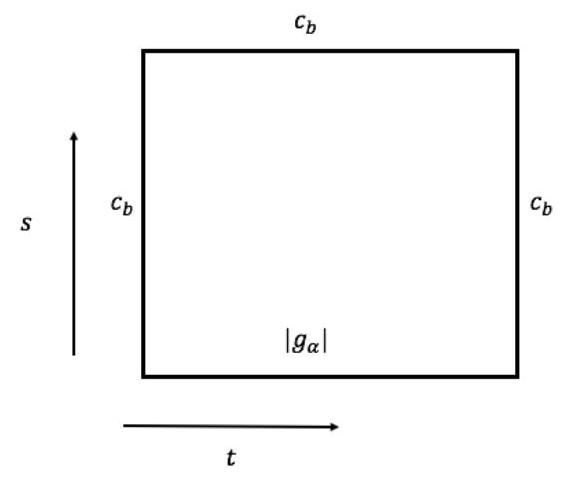
\includegraphics[max width=0.4\textwidth]{images/bo_d2bcsrref24c73avs720_131_681_1563_562_478_0.jpg}
\end{center}
\hspace*{3em} 

Figure 13.1: Graphic illustration for \(H : I \times  I \rightarrow  \left| K\right|\)

Now apply the simplicial approximation theorem, there exists a subdivision of

\(I \times  I\) , denoted as \({\left( I \times  I\right) }_{\left( r\right) }\) (for sufficiently large \(r\) ), shown in the Fig. (13.9)

\begin{center}
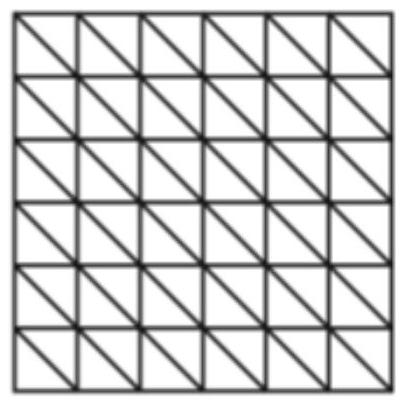
\includegraphics[max width=0.3\textwidth]{images/bo_d2bcsrref24c73avs720_132_636_463_400_400_0.jpg}
\end{center}
\hspace*{3em} 

Figure 13.2: Graphic illustration for \({\left( I \times  I\right) }_{\left( r\right) }\) . In particular, divide \(I \times  I\) into \({r}^{2}\) congruent squares, and then further divide each of these squares along the diagonal to form \({\left( I \times  I\right) }_{\left( r\right) }\) .

such that \(\left| {\left( I \times  I\right) }_{\left( r\right) }\right|  = I \times  I\) , and there exists the simplicial map

\[
{\left( I \times  I\right) }_{\left( r\right) } \rightarrow  K
\]

\[
\text{ such that }\left| G\right|  \simeq  H\text{ . }
\]

Without loss of generality, assume \(r\) is a sufficiently large multiple of \(n\) .

The graphic illustration of \(\left| G\right|\) is shown in Fig. (13.3):

\begin{center}
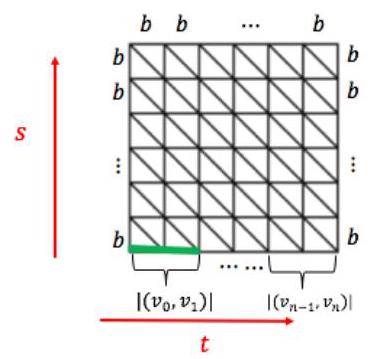
\includegraphics[max width=0.3\textwidth]{images/bo_d2bcsrref24c73avs720_132_594_1549_371_359_0.jpg}
\end{center}
\hspace*{3em} 

Figure 13.3: Graphic illustration for the mapping \(\left| G\right|\) .

In particular, \(\left| G\right|\) maps \(\{ 0,1\}  \times  I\) into \(\{ b\} ;I \times  \{ 1\}\) into \(\{ b\} ;\left( {i/n,0}\right)\) into \(\left\{  {v}_{i}\right\}  ,i =\)

\(0,\ldots ,n\) , and \(\left\lbrack  {i/n,\left( {i + 1}\right) /n}\right\rbrack\) into \(\left| \left( {{v}_{i},{v}_{i + 1}}\right) \right| ,i = 0,\ldots ,n - 1\) .

\begin{itemize}
\item Consider the simplicial subcomplex of \({\left( I \times  I\right) }_{\left( r\right) }\) shown in Fig. (13.4)
\end{itemize}

\begin{center}
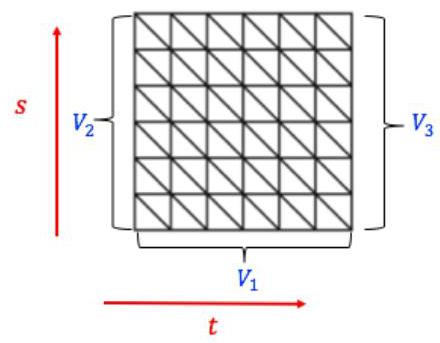
\includegraphics[max width=0.3\textwidth]{images/bo_d2bcsrref24c73avs720_133_744_505_440_343_0.jpg}
\end{center}
\hspace*{3em} 

Figure 13.4: Graphic illustration for the simplicial subcomplex \({V}_{1},{V}_{2},{V}_{3}\) .

For instance, \({V}_{1}\) has \(\left( {r + 1}\right) 0\) -simplicies and \({r1}\) -simplies. It follows that

\[
H\left( \left| {V}_{1}\right| \right)  = H\left( \left| {V}_{2}\right| \right)  = H\left( \left| {V}_{3}\right| \right)  = \{ b\} .
\]

By proposition (10.6), we can pick \(G\) be such that

\[
G\left( {V}_{1}\right)  = G\left( {V}_{2}\right)  = G\left( {V}_{3}\right)  = \{ b\} .
\]

Consider \({W}_{1}\) as the simplicial subcomplex of \({\left( I \times  I\right) }_{\left( r\right) }\) given by the green line shown in Fig. (13.3), which follows that

\[
H\left( \left| {W}_{1}\right| \right)  = \left\{  {{v}_{0},{v}_{1}}\right\}   \Rightarrow  G\left( {W}_{1}\right)  = \left\{  {{v}_{0},{v}_{1}}\right\}
\]

Similarly,

\[
H\left( \left| {W}_{i}\right| \right)  = \left\{  {{v}_{i - 1},{v}_{i}}\right\}   \Rightarrow  G\left( {W}_{i}\right)  = \left\{  {{v}_{i - 1},{v}_{i}}\right\}  ,\forall 1 \leq  i \leq  n.
\]

As a result, \(\left| G\right| \left( \left| {V}_{1}\right| \right)  = \beta  \mathrel{\text{ := }} \left( {b{v}_{0}\cdots {v}_{0}{v}_{1}\cdots {v}_{1}\cdots {v}_{n}\cdots {v}_{n}b}\right)\) , and clearly,

\[
\beta  \sim  \left( {b{v}_{0}{v}_{1}{v}_{2}\cdots {v}_{n - 1}{v}_{n}b}\right)
\]

\[
\sim  \left( {b{v}_{1}{v}_{2}\cdots {v}_{n - 1}b}\right)  = \alpha
\]

\begin{itemize}
\item Now it suffices to show \(\beta  \simeq  e\) . This is true by the sequence of elementary contractions and expansions as shown in the Fig. (13.5).
\end{itemize}

\begin{center}
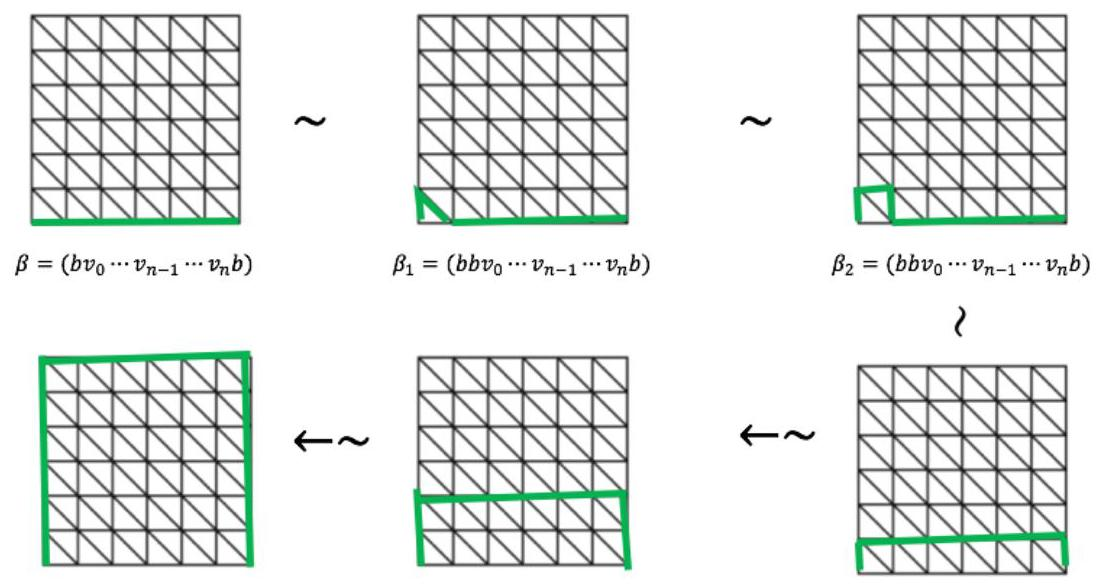
\includegraphics[max width=0.9\textwidth]{images/bo_d2bcsrref24c73avs720_134_260_446_1103_584_0.jpg}
\end{center}
\hspace*{3em} 

Figure 13.5: A sequence of elementary contractions and expansions to show that \(\beta  \sim  \left( {b\cdots b}\right)  = \left( b\right)\) .

The definition of \(E\left( {K,b}\right)\) only involves \(n\) -simplicials for \(n \leq  2\) .

Proposition 13.4 For any simplicial complex \(K\) , consider the simplicial subcomplex \({\operatorname{Skel}}^{n}\left( K\right)  = \left( {{V}_{k},{\sum }_{K}^{n}}\right)\) , where \({\sum }_{K}^{n}\) consists of \(\sigma  \in  {\sum }_{K}\) with \(\left| \sigma \right|  \leq  n + 1\) (this is the \(n\) -skeleton of \(K\) ). Then

\[
{\pi }_{1}\left( {\left| K\right| ,b}\right)  \cong  {\pi }_{1}\left( {\left| {{\operatorname{Skel}}^{2}\left( K\right) }\right| ,b}\right)
\]

Proof. Since \(E\left( {K,b}\right)\) only involves \(n\) -simplicials for \(n \leq  2\) , we imply \(E\left( {K,b}\right)  \cong  E\left( {{\operatorname{Skel}}^{2}\left( K\right) ,b}\right)\) .

Moreover, \({\pi }_{1}\left( {\left| K\right| ,b}\right)  \cong  E\left( {K,b}\right)\) and \({\pi }_{1}\left( {\left| {{\operatorname{Skel}}^{2}\left( K\right) }\right| ,b}\right)  \cong  E\left( {{\operatorname{Skel}}^{2}\left( K\right) ,b}\right)\) .

The proof is complete.

Corollary 13.2 For \(n \geq  2,{\pi }_{1}\left( {S}^{n}\right)\) is a trivial fundamental group.

Proof. Consider the simplicial complex \(K\) with

\[
V = \{ 1,2,\ldots ,n + 2\} ,\;\sum  = \{ \text{ all proper subsets of }V\}
\]

It’s clear that \(\left| K\right|  \cong  {S}^{n}\) , and \({\operatorname{Skel}}^{2}\left( K\right)\) has

\begin{itemize}
\item \(V : \{ 1,\ldots ,n + 2\}\)
\end{itemize}

\begin{itemize}
\item \({\sum }^{2}\) : all subsets of \(V\) with less or equal to 3 elements.
\end{itemize}

For any edge loop \(a\) in \({\pi }_{1}\left( \left| {{\operatorname{skel}}^{2}\left( K\right) }\right| \right)\) , we have

\[
a = \left( {b{v}_{0}{v}_{1}{v}_{2}\cdots {v}_{n}}\right)
\]

\[
\sim  \left( {b{v}_{1}{v}_{2}\cdots {v}_{n - 2}{v}_{n - 1}b}\right)
\]

-...

\[
\sim  \left( b\right)
\]

Therefore, all edge loops \(\alpha\) in \({\pi }_{1}\left( \left| {{\operatorname{skel}}^{2}\left( K\right) }\right| \right)\) satisfies \(\left\lbrack  \alpha \right\rbrack   = \left\lbrack  \left( b\right) \right\rbrack   = e\) ., i.e.,

\[
{\pi }_{1}\left( \left| {{\operatorname{skel}}^{2}\left( K\right) }\right| \right)  \cong  \{ e\}
\]

which implies \({\pi }_{1}\left( \left| K\right| \right)  \cong  {\pi }_{1}\left( \left| {{\operatorname{skel}}^{2}\left( K\right) }\right| \right)  \cong  \{ e\}\) . Since \(\left| K\right|  \cong  {S}^{n}\) , we imply

\[
{\pi }_{1}\left( {S}^{n}\right)  \cong  {\pi }_{1}\left( \left| K\right| \right)  \cong  \{ e\} .
\]

The Corollary (13.2) does not hold for \({S}^{1}\) since the constructed \({\sum }^{2}\) for \({S}^{1}\) does not contain \(\{ 1,2,3\}\) .

Theorem 13.4 \({\pi }_{1}\left( {S}^{1}\right)  \cong  \mathbb{Z}\) . Proof. Construct the triangle \(K\) shown in Fig. (13.6), and it’s clear that \(\left| K\right|  \cong  {S}^{1}\) .

\begin{center}
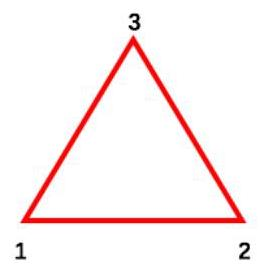
\includegraphics[max width=0.2\textwidth]{images/bo_d2bcsrref24c73avs720_136_687_315_260_269_0.jpg}
\end{center}
\hspace*{3em} 

Figure 13.6: Triangle \(K\) such that \(\left| K\right|  \cong  {S}^{1}\)

It suffices to show \(E\left( {K,1}\right)  \cong  \mathbb{Z}\) . Define the orientation of \(\left| K\right|\) as shown in Fig. (13.7).

\begin{center}
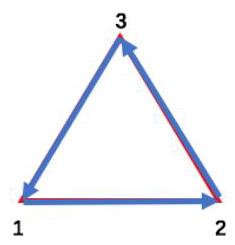
\includegraphics[max width=0.2\textwidth]{images/bo_d2bcsrref24c73avs720_136_695_820_235_245_0.jpg}
\end{center}
\hspace*{3em} 

Figure 13.7: Orientation of \(\left| K\right|\)

Any edge loop \(\alpha\) based at 1 is equivalent to the canonical form

\[
\alpha  \sim  \left( {{1bc1bc}\cdots {1bc1}}\right) ,\;\text{ where }{bc} = {32}\text{ or 23 . }
\]

We construct the isomorphism between \(E\left( {K,b}\right)\) and \(\mathbb{Z}\) directly:

\(\phi  : \;E\left( {K,b}\right)  \rightarrow  \mathbb{Z}\)

with \(\left\lbrack  \alpha \right\rbrack   \mapsto\) winding number of \(\alpha\)

where the winding number of \(\alpha\) is the number of times it traverses(2,3)in the forwards direction minus the number of times it traverses(3,2)in the backwards direction.

The difficult part is to show the well-definedness of \(\phi\) , which can be done by using canonical form of \(\alpha\) .

\section*{13.6. Wednesday for MAT4002}

\section*{13.6.1. Applications on the isomorphism of fundamental group}

Theorem 13.6

\[
{\pi }_{1}\left( {S}^{1}\right)  \cong  \left( {\mathbb{Z}, + }\right)
\]

Proof. Define the orientation of \(\left| K\right|\) as shown in Fig. (13.10).

\begin{center}
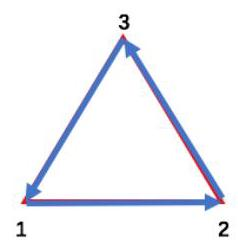
\includegraphics[max width=0.2\textwidth]{images/bo_d2bcsrref24c73avs720_137_692_1023_238_246_0.jpg}
\end{center}
\hspace*{3em} 

\section*{Figure 13.10: Orientation of \(\left| K\right|\)}

Following the proof during last lecture, we construct

\(\phi  : \;E\left( {K,1}\right)  \rightarrow  \left( {\mathbb{Z}, + }\right)\)

with \(\left\lbrack  \alpha \right\rbrack   \mapsto\) winding number of \(\alpha\)

where the winding number of \(\alpha\) is the

number of 23 appearing in \(\alpha\) - number of 32 appearing in \(\alpha\) .

Note that

1. The winding number is invariant under elementary contraction and elementary expansion.

winding number for \(\left( {1\;{23}\cdots {123}\;1}\right)  = m\)

23 shows for \(m\) times

winding number for \(\left( {1\;{32}\cdots {132}\;1}\right)  =  - n\)

32 shows for \(n\) times

3. For any given \(\alpha\) , it is equivalent to a unique (123123...1231) or (132...1321), since otherwise \(\alpha\) will have different winding numbers.

Therefore,(1) and (3) shows the well-definedness of \(\phi\) . In particular,(1) shows that as \(\alpha  \sim  {\alpha }^{\prime }\) , we have \(\phi \left( \left\lbrack  \alpha \right\rbrack  \right)  = \phi \left( \left\lbrack  {\alpha }^{\prime }\right\rbrack  \right)\) ; (2) shows that the winding number of \(\alpha\) is an unique integer.

\begin{itemize}
\item Homomorphism: For given any two edge loops \(\alpha ,\beta\) based at 1, suppose that \(\left\lbrack  \alpha \right\rbrack   = \left\lbrack  \left( {{1bc1bc}\cdots {1bc1}}\right) \right\rbrack\) and \(\left\lbrack  \beta \right\rbrack   = \left\lbrack  \left( {{1pq1pq}\cdots {1pq1}}\right) \right\rbrack\) , then
\end{itemize}

\[
\phi \left( {\left\lbrack  \alpha \right\rbrack   \cdot  \left\lbrack  \beta \right\rbrack  }\right)  = \phi \left( \left\lbrack  {\alpha  \cdot  \beta }\right\rbrack  \right)  = \left\lbrack  \left( {{1bc1bc}\cdots {1bc11pq1pq}\cdots {1pq1}}\right) \right\rbrack
\]

Discuss the case for the sign of \(\phi \left( \left\lbrack  \alpha \right\rbrack  \right)\) and \(\phi \left( \left\lbrack  \beta \right\rbrack  \right)\) separately gives the desired result.

\begin{itemize}
\item Surjectivity: for a given \(m \in  \mathbb{Z}\) , construct \(\alpha\) such that \(\phi \left( \left\lbrack  \alpha \right\rbrack  \right)  = m\) is easy.
\end{itemize}

\begin{itemize}
\item Injectivity: suppose that \(\phi \left( \left\lbrack  \alpha \right\rbrack  \right)  = 0\) , then by definition of \(\phi ,\left\lbrack  \alpha \right\rbrack   = \left\lbrack  \left( 1\right) \right\rbrack   = e\) , which is the trivial element in \(E\left( {K,1}\right)\) .
\end{itemize}

Therefore, \(\phi\) is an isomorphism.

R Actually, we can show that the loop based at 1 given by:

\[
\ell \;I \rightarrow  {S}^{1}
\]

\[
\text{ with }t \mapsto  {e}^{2\pi it}
\]

is a generator for \({\pi }_{1}\left( {{S}^{1},1}\right)\) :

\begin{itemize}
\item \(\phi \left( \left\lbrack  \ell \right\rbrack  \right)  = 1\) , where \(\phi  : {\pi }_{1}\left( {{S}^{1},1}\right)  \cong  \mathbb{Z}\) .
\end{itemize}

\begin{itemize}
\item The loop
\end{itemize}

\[
{\ell }^{m} : \;I \rightarrow  {S}^{1}\;m \in  \mathbb{Z}
\]

\[
\text{ with }{\ell }^{m}\left( t\right)  = {e}^{2\pi imt}
\]

gives \(\phi \left( \left\lbrack  {\ell }^{m}\right\rbrack  \right)  = m\)

Corollary 13.4 [Fundamental Theorem of Algebra] All non-constant polynomials in \(\mathbb{C}\) has at least one root in \(\mathbb{C}\)

Proof. - Suppose on the contrary that

\[
p\left( x\right)  = {a}_{n}{x}^{n} + \cdots  + {a}_{1}x + {a}_{0}{a}_{n} \neq  0
\]

has no roots, then \(p\) is a mapping from \(\mathbb{C}\) to \(\mathbb{C} \smallsetminus  \{ 0\}\) . It’s clear that \(\mathbb{C} \smallsetminus  \{ 0\}  \simeq  \{ z \in\)

\(\mathbb{C} \mid  \left| z\right|  = 1\}\) , and therefore

\[
{\pi }_{1}\left( {\mathbb{C}\smallsetminus \{ 0\} }\right)  = {\pi }_{1}\left( {S}^{1}\right)  \cong  \mathbb{Z}.
\]

\begin{itemize}
\item The induced homomorphism \({p}^{ * }\) of \(p\) is given by:
\end{itemize}

\[
{p}_{ * } : \;{\pi }_{1}\left( \mathbb{C}\right)  \rightarrow  {\pi }_{1}\left( {\mathbb{C}\smallsetminus \{ 0\} }\right)
\]

\[
\text{ with }\{ e\}  \mapsto  \mathbb{Z}
\]

Note that \({\pi }_{1}\left( \mathbb{C}\right)\) is trival as \(\mathbb{C}\) is contractible. Also, \({p}_{ * }\left( e\right)  = 0\) .

\begin{itemize}
\item Consider the inclusion from \({C}_{r} = \{ z \in  \mathbb{C}\left| \right| z \mid   = r\}\) to \(\mathbb{C}\) :
\end{itemize}

\(i : \;{C}_{r} \rightarrow  \mathbb{C}\)

with \(z \mapsto  z\)

It satisfies the diagram given below: Or equivalently,

\begin{center}
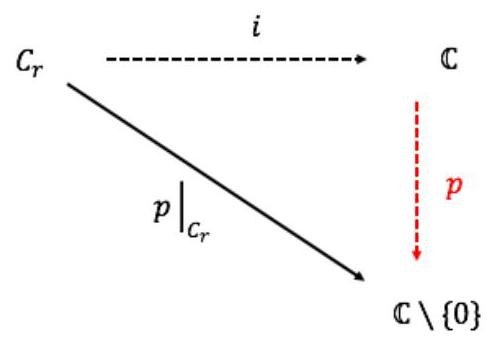
\includegraphics[max width=0.4\textwidth]{images/bo_d2bcsrref24c73avs720_140_723_324_495_359_0.jpg}
\end{center}
\hspace*{3em} 

As a result, the induced homomorphism \({i}^{ * }\) of \(i\) satisfies the diagram

\begin{center}
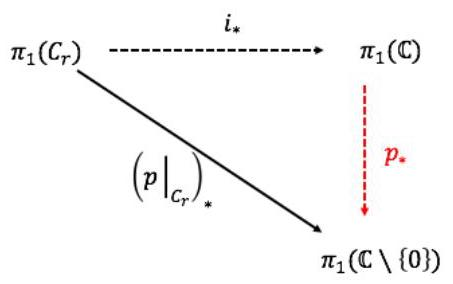
\includegraphics[max width=0.3\textwidth]{images/bo_d2bcsrref24c73avs720_140_723_888_453_284_0.jpg}
\end{center}
\hspace*{3em} 

\begin{center}
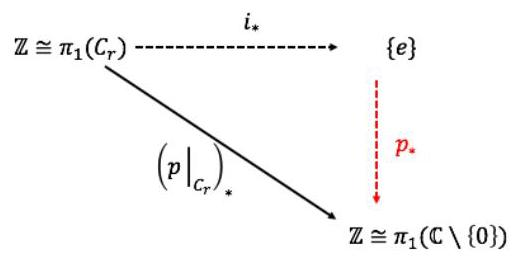
\includegraphics[max width=0.4\textwidth]{images/bo_d2bcsrref24c73avs720_140_722_1373_516_261_0.jpg}
\end{center}
\hspace*{3em} 

Therefore, \({p}_{ * } \circ  {i}_{ * }\) is a zero map since \({p}_{ * }\left( e\right)  = 0\) , i.e., \({\left( {\left. p\right| }_{{C}_{r}}\right) }_{ * }\) is a zero homomorphism.

\begin{itemize}
\item Then it’s natural to study \({\left. p\right| }_{{C}_{r}} : {C}_{r} \rightarrow  \mathbb{C} \smallsetminus  \{ 0\}\) . Construct
\end{itemize}

\[
\left\{  \begin{array}{l} q\left( z\right)  = k \cdot  {z}^{n},\;k \mathrel{\text{ := }} \frac{p\left( r\right) }{{r}^{n}}\text{ is a constant } \\  p\left( z\right)  = {a}_{n}{z}^{n} + \cdots  + {a}_{1}z + {a}_{0} \end{array}\right.
\]

Therefore, \(p\left( r\right)  = q\left( r\right)\) , and \({\left. p\right| }_{{C}_{r}},{\left. q\right| }_{{C}_{r}} : {C}_{r} \rightarrow  \mathbb{C} \smallsetminus  \{ 0\}\) .

\begin{itemize}
\item We claim that \({\left. p\right| }_{{C}_{r}} \simeq  {\left. q\right| }_{{C}_{r}}\) for large \(r\) . First construct the mapping
\end{itemize}

\[
H : \;{C}_{r} \times  \left\lbrack  {0,1}\right\rbrack   \rightarrow  \mathbb{C}
\]

\[
\text{ with }H\left( {z,t}\right)  = {tp}\left( z\right)  + \left( {1 - t}\right) q\left( z\right)
\]

\[
\text{ and }\;H\left( {z,0}\right)  = q\left( z\right) ,H\left( {z,1}\right)  = p\left( z\right)
\]

If we want to show \(H\) is the homotopy between \({\left. p\right| }_{{C}_{r}}\) and \({\left. q\right| }_{{C}_{r}}\) , it suffices to

show that \(H\) is well-defined, i.e., \(H : {C}_{r} \times  \left\lbrack  {0,1}\right\rbrack   \rightarrow  \mathbb{C} \smallsetminus  \{ 0\}\) .

Suppose on the contrary that there exists(z, t)such that

\[
\left( {1 - t}\right) p\left( z\right)  + {tq}\left( z\right)  = 0,\;\left| z\right|  = r,t \in  \left\lbrack  {0,1}\right\rbrack
\]

Or equivalently,

\[
\left( {1 - t}\right) \left( {{a}_{n}{z}^{n} + \cdots  + {a}_{1}z + {a}_{0}}\right)  + t \cdot  k{z}^{n} = 0.
\]

Substituting \(k\) with \(p\left( r\right) /{r}^{n}\) gives

\[
{a}_{n}{z}^{n} + \cdots  + {a}_{1}z + {a}_{0} = t\left( {{a}_{n - 1}{z}^{n - 1} + \cdots  + {a}_{0} - {a}_{n - 1}\frac{{z}^{n}}{r} - \cdots  - {a}_{1}\frac{{z}^{n}}{{r}^{n - 1}} - {a}_{0}\frac{{z}^{n}}{{r}^{n}}}\right)
\]

The LHS has leading order \(n\) , while the RHS has leading order less or equal to \(n - 1\) . As \(r = \left| z\right|  \rightarrow  \infty ,t \rightarrow  \infty\) . Therefore, the equality does not hold in the range \(t \in  \left\lbrack  {0,1}\right\rbrack\) when \(r\) is sufficiently large.

For this choice of \(r = \left| z\right|\) ,

\[
H : {C}_{r} \times  \left\lbrack  {0,1}\right\rbrack   \rightarrow  \mathbb{C} \smallsetminus  \{ 0\}
\]

gives the homotopy \({\left. p\right| }_{{C}_{r}} \simeq  {\left. q\right| }_{{C}_{r}}\) .

\begin{itemize}
\item Therefore, we imply \({\left( {\left. p\right| }_{{C}_{r}}\right) }_{ * } = {\left( {\left. q\right| }_{{C}_{r}}\right) }_{ * }\) . Now we check the mapping \({\left( {\left. q\right| }_{{C}_{r}}\right) }_{ * } : \mathbb{Z} \rightarrow  \mathbb{Z}\) . In particular, we check the value of \({\left( {\left. q\right| }_{{C}_{r}}\right) }_{ * }\left( 1\right)\) , where 1 is the generator in \({\pi }_{1}\left( {C}_{r}\right)\) .
\end{itemize}

Here we construct the loop

\[
\ell  : \;I \rightarrow  {C}_{r}
\]

\[
\text{ with }\ell \left( t\right)  = r{e}^{2\pi it}
\]

and therefore \(\left\lbrack  \ell \right\rbrack   = 1\) . It follows that

\[
{\left( {\left. q\right| }_{{C}_{r}}\right) }_{ * }\left( 1\right)  = {\left( {\left. q\right| }_{{C}_{r}}\right) }_{ * }\left( \left\lbrack  \ell \right\rbrack  \right)  = \left\lbrack  {{\left. q\right| }_{{C}_{r}}\left( \ell \right) }\right\rbrack   = q\left( {r{e}^{2\pi it}}\right)  = k \cdot  {r}^{n} \cdot  {e}^{2\pi int} \neq  0.
\]

Therefore, \({\left( {\left. q\right| }_{{C}_{r}}\right) }_{ * }\) is not a zero homomorphism, i.e., \({\left( {\left. q\right| }_{{C}_{r}}\right) }_{ * } : \mathbb{Z} \cong  {\pi }_{1}\left( {C}_{r}\right)  \rightarrow  {\pi }_{1}\left( {C\{ 0\} }\right)  \cong\)  \(\mathbb{Z}\) is the map \(1 \mapsto  n\) , which gives a contradiction.

\section*{14.3. Monday for MAT4002}

\section*{14.3.1. Fundamental group of a Graph}

Definition 14.3 [Graph] A graph \(T = \left( {V,E}\right)\) is defined by the following components:

\begin{itemize}
\item \(V\) is a finite or countable set, called vertex set;
\end{itemize}

\begin{itemize}
\item \(E\) is a finite or countable set, called edge set;
\end{itemize}

\begin{itemize}
\item A function \(\delta  : E \rightarrow  V \times  V\) with \(\delta \left( e\right)  = \left( {\ell \left( e\right) ,\tau \left( e\right) }\right)\) , where \(\ell \left( e\right) ,\tau \left( e\right)\) is known as the endpoints of \(e\) .
\end{itemize}

\begin{itemize}
\item Example 14.2 1. Let \(V = \{ 1\} ,E = \left\{  {{e}_{1},{e}_{2},{e}_{3}}\right\}\) , and define \(\delta \left( {e}_{i}\right)  = \left( {1,1}\right) ,i = 1,2,3\) . The graph(V, E)is represented below:
\end{itemize}

\begin{center}
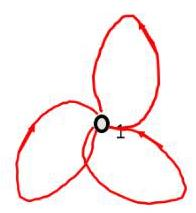
\includegraphics[max width=0.2\textwidth]{images/bo_d2bcsrref24c73avs720_143_735_1203_196_213_0.jpg}
\end{center}
\hspace*{3em} 

2. Let \(V = \left\{  {{e}_{1},{e}_{2},{e}_{3}}\right\}\) and \(E = \left\{  {{e}_{1},\ldots ,{e}_{6}}\right\}\) , and define

\[
\delta \left( {e}_{1}\right)  = \left( {1,1}\right) ,\;\delta \left( {e}_{2}\right)  = \left( {1,2}\right) ,\;\delta \left( {e}_{3}\right)  = \left( {1,2}\right) ,
\]

\[
\delta \left( {e}_{4}\right)  = \left( {2,3}\right) ,\;\delta \left( {e}_{5}\right)  = \left( {2,3}\right) ,\;\delta \left( {e}_{6}\right)  = \left( {3,3}\right) .
\]

The graph(V, E)is represented below (We do not care the direction of edges for this graph):

\begin{center}
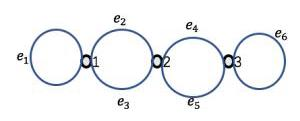
\includegraphics[max width=0.2\textwidth]{images/bo_d2bcsrref24c73avs720_143_688_1907_300_121_0.jpg}
\end{center}
\hspace*{3em} 

Definition 14.4 [Realizatin of a Graph] For a given graph \(\Gamma  = \left( {V,E}\right)\) , construct a realization by

\[
\{ \left| V\right|  \times  \{ \text{ zero simplies }\} \coprod \left| E\right|  \times  \{ 1\text{ -simplies }\} \} / \sim
\]

where the equivalence class is induced from the function \(\delta\) . We still call this realization of the graph as \(\Gamma\) .

In general, graphs are not simplicial complexes. But we can "sub-divide" each edge of \(\Gamma\) into three parts such that there exists simplicial complex \(K\) with \(\left| K\right|  \cong  \Gamma\) . For instance,

\begin{center}
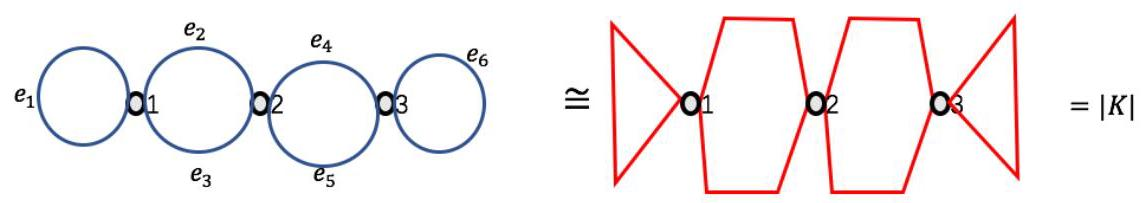
\includegraphics[max width=0.9\textwidth]{images/bo_d2bcsrref24c73avs720_144_387_976_1147_203_0.jpg}
\end{center}
\hspace*{3em} 

where \(\left| K\right|\) is a simplicial complex.

\begin{itemize}
\item Subgraph \({\Gamma }^{\prime } \subseteq  \Gamma  : {\Gamma }^{\prime } = \left( {{V}^{\prime },{E}^{\prime }}\right)\) with \({V}^{\prime } \subseteq  V\) and \({E}^{\prime } \subseteq  E\) , and
\end{itemize}

\[
\delta { \mid  }_{{V}^{\prime }} : {E}^{\prime } \rightarrow  {V}^{\prime } \times  {V}^{\prime }
\]

\begin{itemize}
\item Edge path: A continous function \(p : \left\lbrack  {0,1}\right\rbrack   \rightarrow  \Gamma\) such that there exists \(n \in  \mathbb{N}\) satisfying
\end{itemize}

\[
{\left. p\right| }_{\left\lbrack  i/n,i + 1/n\right\rbrack  } : \left\lbrack  {\frac{i}{n},\frac{i + 1}{n}}\right\rbrack   \rightarrow  T
\]

is a path along an edge of \(\Gamma\) , or a constant function on a vertex of \(\Gamma\) , for \(0 \leq  i \leq  n - 1\) .

Under the homeomorphism \(\Gamma  \cong  \left| K\right|\) , each edge path is homotopic to

\(\left| {g}_{\alpha }\right|\) for some edge path \(\alpha\) in the simplicial complex \(K\) . For instance,

\begin{center}
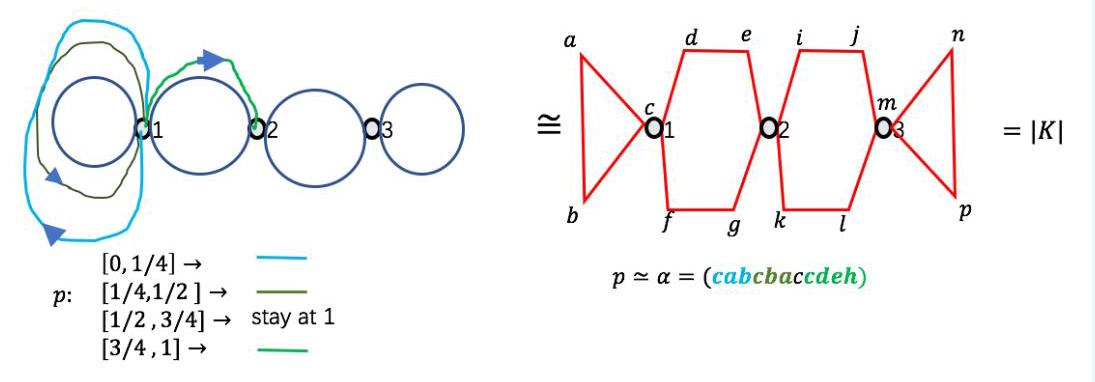
\includegraphics[max width=0.9\textwidth]{images/bo_d2bcsrref24c73avs720_145_296_329_1095_382_0.jpg}
\end{center}
\hspace*{3em} 

\begin{itemize}
\item An Edge loop is an edge path \(p\) such that \(p\left( 0\right)  = p\left( 1\right)  = b \in  V\) .
\end{itemize}

\begin{itemize}
\item Embedded Edge Loop: An injective edge loop, i.e., \(p : \left\lbrack  {0,1}\right\rbrack   \rightarrow  \Gamma\) such that
\end{itemize}

for \(x \notin  V,\;{p}^{-1}\left( x\right)  = \varnothing\) or a single point.

\begin{itemize}
\item Tree: a connected graph \(T\) that contains no embedded edge loop \(p : \left\lbrack  {0,1}\right\rbrack   \rightarrow  T\) . For instance, as shown in the figure, \({T}_{1}\) contains no edge loop, in particular, the edge loop(a, b, a)is not embedded; \({T}_{2}\) contains embedded edge loop(a, b, c, d, a).
\end{itemize}

\begin{itemize}
\item Maximal Tree of a connected graph \(\Gamma\) :
\end{itemize}

\begin{itemize}
\item A subgraph \(T\) of \(\Gamma\) such that \(T\) is a tree.
\end{itemize}

\begin{itemize}
\item By adding an edge \(e \in  E\left( \Gamma \right)  \smallsetminus  E\left( T\right)\) into \(T\) , the new graph is no longer a tree. For instance, \(T \subseteq  \Gamma\) shown in the figure below is a maximal tree.
\end{itemize}

\begin{center}
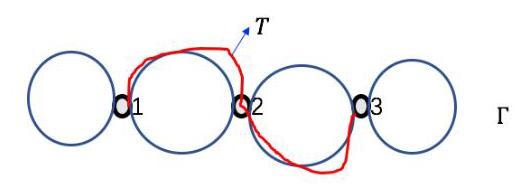
\includegraphics[max width=0.4\textwidth]{images/bo_d2bcsrref24c73avs720_145_580_1689_526_186_0.jpg}
\end{center}
\hspace*{3em} 

Theorem 14.5 Let \(\Gamma\) be a connected graph, and \(T\) is a subgraph of \(\Gamma\) such that \(T\) is a tree. Then \(T\) is a maximal tree if and only if \(V\left( T\right)  = V\left( \Gamma \right)\) .

Moreover, there always exists a maximal tree for all \(\Gamma\) .

Proof Outline for second part. Construct an ordering of \(\left\{  {{v}_{1},\ldots ,{v}_{i}}\right\}   \subseteq  V\left( \Gamma \right)\) , such that for each integer \(i \geq  2\) , there is an edge connecting \({v}_{i + 1}\) with some vertex in \(\left\{  {{v}_{1},\ldots ,{v}_{i}}\right\}\) .

Then construct \({T}_{1} \subseteq  {T}_{2} \subseteq  \cdots\) , where \({T}_{i}\) is a tree containing vertices \(\left\{  {{v}_{1},\ldots ,{v}_{i}}\right\}\) . As a result, \(T = { \cup  }_{i \in  \mathbb{N}}{T}_{i}\) is a maximal tree.

Theorem 14.6 Let \(\Gamma\) be a connected graph. Then \(\pi \left( \Gamma \right)\) is isomorphic to the free group generated by \(\# \{ E\left( \Gamma \right)  \smallsetminus  E\left( T\right) \}\) elements, for any maximal tree of \(\Gamma\) .

1. The graph \(T \subseteq  {\Gamma }_{1}\) shown in the figure below is a maximal tree.

\begin{center}
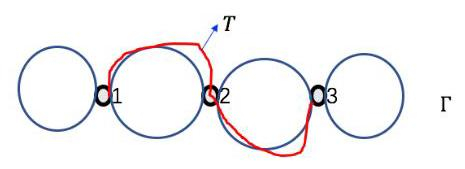
\includegraphics[max width=0.3\textwidth]{images/bo_d2bcsrref24c73avs720_146_760_1090_465_169_0.jpg}
\end{center}
\hspace*{3em} 

Therefore, \({\pi }_{1}\left( {\Gamma }_{1}\right)  \cong  \langle a,b,c,d\rangle\) since \(\# \left\{  {E\left( {\Gamma }_{1}\right)  \smallsetminus  E\left( T\right) }\right\}   = 4\) .

2. The graph \(T \subseteq  {\Gamma }_{2}\) shown in the figure below is a maximal tree.

\begin{center}
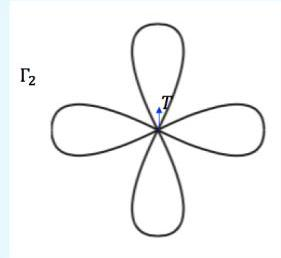
\includegraphics[max width=0.2\textwidth]{images/bo_d2bcsrref24c73avs720_146_832_1473_281_258_0.jpg}
\end{center}
\hspace*{3em} 

Therefore, \({\pi }_{1}\left( {\Gamma }_{2}\right)  \cong  \langle a,b,c,d\rangle\) since \(\# \left\{  {E\left( {\Gamma }_{2}\right)  \smallsetminus  E\left( T\right) }\right\}   = 4\) .

3. Note that \({\Gamma }_{1} \simeq  {\Gamma }_{2}\) . The reason for such homotopy equivalence is in the link

https://www.math3ma.com/blog/clever-homotopy-equivalences

\section*{15.3. Monday for MAT4002}

Theorem 15.4 Let \(\Gamma\) be a connected graph. Then \(\pi \left( \Gamma \right)\) is isomorphic to the free group generated by \(\# \{ E\left( \Gamma \right)  \smallsetminus  E\left( T\right) \}\) elements, for any maximal tree of \(\Gamma\) .

Now we give a proof for this theorem on one special case of \(\Gamma\) :

\begin{center}
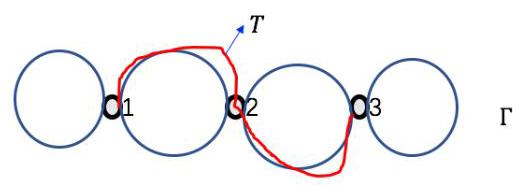
\includegraphics[max width=0.4\textwidth]{images/bo_d2bcsrref24c73avs720_147_728_630_521_185_0.jpg}
\end{center}
\hspace*{3em} 

Proof. \(\; \bullet\) Fix an orientation for each \(e \in  E\left( \Gamma \right)  \smallsetminus  E\left( T\right)\) :

\begin{center}
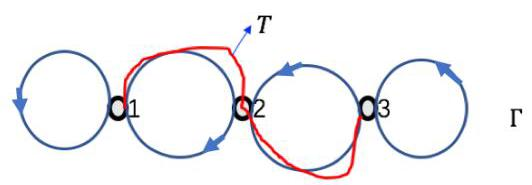
\includegraphics[max width=0.4\textwidth]{images/bo_d2bcsrref24c73avs720_147_704_1012_532_185_0.jpg}
\end{center}
\hspace*{3em} 

\begin{itemize}
\item Now let \(K\) be a simplicial complex with \(\left| K\right|  \cong  \Gamma\) :
\end{itemize}

\begin{center}
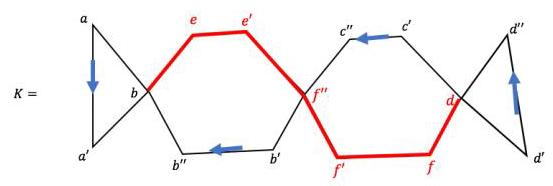
\includegraphics[max width=0.4\textwidth]{images/bo_d2bcsrref24c73avs720_147_695_1382_553_186_0.jpg}
\end{center}
\hspace*{3em} 

As a result, \(E\left( {K,b}\right)  \cong  {\pi }_{1}\left( \Gamma \right)\)

\begin{itemize}
\item Now we construct the group homomorphism
\end{itemize}

\[
\phi  : \;\langle \alpha ,\beta ,\gamma ,\delta \rangle  \rightarrow  E\left( {K,b}\right)
\]

\[
\text{ with }\phi \left( \alpha \right)  = \left\lbrack  {b{a}^{\prime }{a}^{\prime \prime }b}\right\rbrack
\]

\[
\phi \left( \beta \right)  = \left\lbrack  {{be}{e}^{\prime }{f}^{\prime \prime }{b}^{\prime }{b}^{\prime \prime }b}\right\rbrack
\]

\[
\phi \left( \gamma \right)  = \left\lbrack  {{be}{e}^{\prime }{f}^{\prime \prime }{f}^{\prime }{fd}{c}^{\prime }{c}^{\prime \prime }{f}^{\prime \prime }{e}^{\prime }{eb}}\right\rbrack
\]

\[
\phi \left( \delta \right)  = \left\lbrack  {{\text{ bee }}^{\prime }{f}^{\prime \prime }{f}^{\prime }{fd}{d}^{\prime \prime }{d}^{\prime }{df}{f}^{\prime }{f}^{\prime \prime }{e}^{\prime }{eb}}\right\rbrack
\]

\begin{itemize}
\item We can show the group homomorphism \(\phi\) is bijective. In particular, the inverse of \(\phi\) is given by:
\end{itemize}

\[
\Psi  : \;E\left( {K,b}\right)  \rightarrow  \langle \alpha ,\beta ,\gamma ,\delta \rangle
\]

where for any \(\left\lbrack  \ell \right\rbrack   \mathrel{\text{ := }} \left\lbrack  {b{v}_{1}\cdots {v}_{n}}\right\rbrack   \in  E\left( {K,b}\right)\) , the mapping \(\Psi \left\lbrack  \ell \right\rbrack\) is constructed by

(a) Remove all other letters appearing in \(\ell\) except \(b,{a}^{\prime },{a}^{\prime \prime },{b}^{\prime },{b}^{\prime \prime },{c}^{\prime },{c}^{\prime \prime },{d}^{\prime },{d}^{\prime \prime }\)

(b) Assign

\[
\alpha ,{\alpha }^{-1},\beta ,{\beta }^{-1},\gamma ,{\gamma }^{-1},\delta ,{\delta }^{-1}
\]

for each appearance of

\[
{a}^{\prime }{a}^{\prime \prime },{a}^{\prime \prime }{a}^{\prime },{b}^{\prime }{b}^{\prime \prime },{b}^{\prime \prime }{b}^{\prime },{c}^{\prime }{c}^{\prime \prime },{c}^{\prime \prime }{c}^{\prime },{d}^{\prime }{d}^{\prime \prime },{d}^{\prime \prime }{d}^{\prime }\text{ , }
\]

respectively.